\section{The Choice of radiation}
	
	week 4, lec - 21 + week 5, lec - 22.
	
The maximum value of $\sin \theta = 1$ $\implies \theta_\mathrm{max} = \SI{90}{\degree}.$

\begin{align}
&\therefore \lambda = 2 \d_{hk\ell}^\mathrm{(min)} ~ \mathrm{for} ~ \theta = \pi/2 \nonumber \\[0.8em]
&\implies \d_{hk\ell}^\mathrm{(min)} = \dfrac{\lambda}{2} = \begin{dcases*}
\dfrac{1.54}{2} = \SI{0.77}{\angstrom} & for $\mathrm{Cu}~K_\alpha$ radiation, \\[0.8em]
\dfrac{0.71}{2} = \SI{0.35}{\angstrom} & for $\mathrm{Mo}~K_\alpha$ radiation.
\end{dcases*}
\end{align}

Thus, we see that we get a higher resolution when using $\mathrm{Mo}~K_\alpha$ radiation compared to $\mathrm{Cu}~K_\alpha$ radiation.

According to the standards set by IUCr, for $\mathrm{Mo}~K_\alpha$ radiation, data has to be recorded \ifnt{at least} upto $\SI{50}{\degree}$ in $2\theta$ for an acceptable crystal structure solution.

Substituting $\theta = \SI{25}{\degree}$ in Bragg's Law, for $\mathrm{Mo}~K_\alpha$, we get%
%
\begin{align}
&\phantom{\implies} \SI{0.71}{\angstrom} = 2 d_{hk\ell} \sin \SI{25}{\degree} \nonumber \\
&\implies d_{hk\ell} = \SI{1.183}{\angstrom}.
\end{align}

If we want to achieve this same resolution with $\mathrm{Cu}~K_\alpha,$%
%
\begin{align}
&\phantom{\implies} \SI{1.54}{\angstrom} = 2 \cross \SI{1.2}{\angstrom} \sin \theta \nonumber \\
&\implies \theta = \SI{42}{\degree} \nonumber \\
&\implies 2\theta = \SI{84}{\degree}.
\end{align}

Therefore, we have to record upto a higher angle to achieve the same resolution with $\mathrm{Cu}~K_\alpha.$

\begin{figure}[h!]
	\centering
	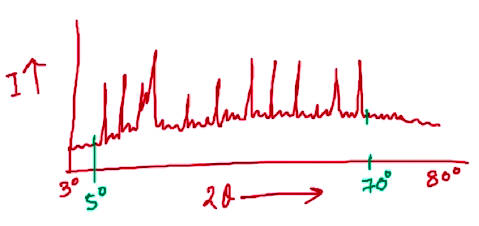
\includegraphics[scale=0.8]{pxrd_peaks.png}
	\caption{\label{fig:pxrd_peaks}Suppose we have recorded PXRD data using $\mathrm{Cu}~K_\alpha$ radiation from $\SI{3}{\degree}$ to $\SI{80}{\degree}$ in $2\theta$. The first peak appears at, say, $\SI{5}{\degree}$ and the last peak at $\SI{70}{\degree}.$ Image taken from \cite[lecture 22]{Chowdhury2022}.}
\end{figure}

Suppose we have a PXRD data as in figure~\ref{fig:pxrd_peaks}. Using Bragg's Law,%
%
\begin{align}
&\phantom{\implies} \dfrac{\lambda_\mathrm{Cu}}{\lambda_\mathrm{Mo}} = \dfrac{2 d_{hk\ell} \sin \theta_\mathrm{Cu}}{2 d_{hk\ell} \sin \theta_\mathrm{Mo}} \nonumber \\[0.8em]
&\implies \dfrac{\sin \theta_\mathrm{Cu}}{\sin \theta_\mathrm{Mo}} = \dfrac{1.54}{0.71}. \label{eq:sin_theta_Cu_Mo}
\end{align}

The first peak is at $\approx \SI{5}{\degree}$ in $2\theta_\mathrm{Cu}$ for $\mathrm{Cu}~K_\alpha$. Using eqn.~\eqref{eq:sin_theta_Cu_Mo}, we find that for $\mathrm{Mo}~K_\alpha,$ it will be at $2\theta_\mathrm{Mo} \approx \SI{2.3}{\degree}.$ Similarly, the last peak, which occurs at $2\theta_\mathrm{Cu} \approx \SI{70}{\degree},$ would have appeared at $2\theta_\mathrm{Mo} \approx \SI{30.66}{\degree}.$

Thus, when the data is recorded using $\mathrm{Cu}~K_\alpha$, the peaks appear in the range $\SI{5}{\degree}$ to $\SI{70}{\degree}$ in $2\theta,$ while for $\mathrm{Mo}~K_\alpha,$ they would have been squeezed between $\SI{2.3}{\degree}$ to $\SI{30.66}{\degree}$ in $2\theta.$ This will reduce the resolution of the peaks, and they may overlap or merge with each other, whereby we will lose information.

For PXRD, synchrotron source gives the best resolution. In the absence of that, we use $\mathrm{Cu}~K_\alpha.$ In SCXRD, where spots appear and they are well resolved, we can use $\mathrm{Mo}~K_\alpha$ radiation for higher resolution.

Note that monochromatic radiation is preferred because if we use polychromatic radiation, for a particular set of planes, there will be peaks for each wavelength in the X-ray diffraction spectrum, which are difficult to separate. In PXRD, however, often, we do not use a monochromator because it reduces the intensity drastically. In that situation, we have to identify the $K_{\alpha_1}$ and the $K_{\alpha_2}$ peaks in the spectra and separate them.